\documentclass{article}

%Russian-specific packages
%--------------------------------------
\usepackage[russian]{babel}
%--------------------------------------

%Hyphenation rules
%--------------------------------------
\usepackage{hyphenat}
%--------------------------------------

%Math
%--------------------------------------
\usepackage{mathtools}
\usepackage{mathrsfs}
\usepackage{amsmath}
\usepackage{amsfonts}
\usepackage{accents}
\usepackage{systeme}
\DeclareMathOperator{\rank}{rank}
\DeclareMathOperator{\im}{im}
\DeclareMathOperator{\sign}{sign}
\newcommand\aug{\fboxsep=-\fboxrule\!\!\!\fbox{\strut}\!\!\!}
%-------------------------------------- 

%Hyperlinks
%--------------------------------------
\usepackage[svgnames]{xcolor}
\usepackage[colorlinks=true, linkcolor=Blue, urlcolor=Blue]{hyperref}
%--------------------------------------

%Graphics
%--------------------------------------
\usepackage{graphicx}
\usepackage{wrapfig}
%--------------------------------------

%errors fix
%--------------------------------------
\usepackage{microtype}
\usepackage[a4paper,left=3cm,right=3cm,top=2cm,bottom=2cm]{geometry}
\usepackage{verbatim}
%--------------------------------------

\begin{document}
\section{Линейное (векторное) пространство. Векторное пространство $\mathbb{R}^m$.}
\subsection{Линейное пространство}
Пусть дано поле $F$. Линейным пространством над полем $F$ называется произвольное не пустое множество $V$, на котором заданы операция сложения, являющаяся Абелевой группой, и операция умножения вектора на любой скаляр из $F$. Умножение на скаляр обладает следующими свойствами:
\begin{itemize}
    \item $x, y \in V \land t \in F \implies t(x + y) = tx + ty$
    \item $t, s \in F \land x \in F \implies (t + s)x = tx + sx$
    \item $t, s \in F \land x \in F \implies t(sx) = (ts)x$
    \item $x \in V \implies 1x = x$
\end{itemize}
\subsection{Векторное пространство $\mathbb{R}^m$}
Теперь определим пространство $\mathbb{R}^m$. Возьмем множество строк вида $(x_1, x_2, \dots, x_m)$, где $x_i \in \mathbb{R}$. Определим операции и сущности. 
\begin{itemize}
    \item Сложение: $(x_1, x_2, \dots, x_m) + (y_1, y_2, \dots, y_m) = (x_1 + y_1, x_2 + y_2, \dots, x_m + y_m)$
    \item $0$: $(0, 0, \dots, 0)$
    \item Умножение на скаляр $t \in \mathbb{R}$: $t(x_1, x_2, \dots, x_m) = (tx_1, tx_2, \dots, tx_m)$
\end{itemize} 
Такое определение очевидным образом будет удовлетворять всем аксиомам линейного пространства.

\section{Метрическое пространство. Метрическое пространство $\mathbb{R}^m$. Метрики $\rho_0$, $\rho_1$ и $\rho_e$, их эквивалентность.}
\subsection{Метрическое пространство}
Метрика на $X$ --- отображение $\rho : X \times X \to \mathbb{R}$, для которого выполняется следующий набор аксиом: 
\begin{itemize}
    \item $\rho(x, y) \geq 0$
    \item $\rho(x, y) = 0 \equiv x = y$
    \item $\rho(x, y) = \rho(y, x)$
    \item $\rho(x, y) \leq \rho(x, z) + \rho(z, y)$
\end{itemize}
Пространство с определенной на нем метрикой называется метрическим. \\
Метрики $\rho_1$ и $\rho_2$ эквивалентны если: 
$\exists a, b \in \mathbb{R}^+ : \forall x, y \in X : a\rho_2(x, y) \leq \rho_1(x, y) \leq b\rho_2(x, y)$.
\begin{itemize}
    \item Рефлексивность очевидна, достаточно взять $a = b = 1$
    \item Докажем симметричность:
    $$
    a\rho_2(x, y) \leq \rho_1(x, y) \leq b\rho_2(x, y) \implies
    a\rho_2(x, y) \leq \rho_1(x, y) \land \rho_1(x, y) \leq b\rho_2(x, y) \implies
    $$
    $$
    \rho_2(x, y) \leq \frac{1}{a}\rho_1(x, y) \land \frac{1}{b}\rho_1(x, y) \leq \rho_2(x, y) \implies \frac{1}{b}\rho_1(x, y) \leq \rho_2(x, y) \leq \frac{1}{a}\rho_1(x, y)
    $$
    \item Докажем транзитивность
    $$
    a\rho_2(x, y) \leq \rho_1(x, y) \leq b\rho_2(x, y) \land c\rho_3(x, y) \leq \rho_2(x, y) \leq d\rho_3(x, y) \implies
    $$
    $$
    ac\rho_3(x,y) \leq a\rho_2(x,y) \leq \rho_1(x,y) \leq b\rho_2(x,y) \leq bd\rho_3(x, y)
    $$
\end{itemize}
\subsection{Метрическое пространство $\mathbb{R}^m$}
Введем несколько метрик в $\mathbb{R}^m$:
\begin{itemize}
    \item $\rho_0(x, y) = \max_{k \in \overline{1, m}} |x_k - y_k|$
    \begin{itemize}
        \item $\rho_0(x, y) \geq 0$ потому что это верно для модуля.
        \item $\rho_0(x,y) = \rho_0(y, x)$ потому что значения под модулем можно поменять местами.
        \item $\rho_0(x, y) = 0 \equiv
        (\forall k \in \overline{1, m} : |x_k - y_k| = 0 \equiv x_k = y_k)
        \equiv x = y$
        \item $\rho_0(x, y) = 
        \max_{k \in \overline{1, m}} |x_k - y_k| \leq
        |x_k - z_k| + |z_k - y_k| \leq
        \max_{i \in \overline{1, m}} |x_i - z_i| + |z_i - y_i| =
        \rho_0(x, z) + \rho_0(z, y)$
    \end{itemize}
    \item $\rho_1(x, y) = \sum_{k \in \overline{1, m}} |x_i - y_i|$
    \begin{itemize}
        \item $\rho_1(x, y) \geq 0$ сумма положительных величин
        \item $\rho_1(x,y) = \rho_p(y, x)$ аналогично $\rho_0$
        \item $\rho_1(x, y) = 0$ аналогично $\rho_0$
        \item $\rho_1(x, y) = \rho_e(x, z) + \rho_e(z, y)$ следует из правила треугольника для модуля
    \end{itemize}
    \item $\rho_e(x, y)$ --- Евклидова метрика. Задается в любом Евклидовом пространстве как $\rho_e(x, y) = \sqrt{(x-y) \circ (x-y)}$ где точка --- скалярное произведение.
    \begin{itemize}
        \item Корректность этой метрики будет доказана далее.
    \end{itemize}
    \item В частном случае, если скалярное произведение определить как сумму покомпонентных произведений: $x \circ y = x_1y_1 + x_2y_2 + \dots + x_my_m$, то эта метрика примет вид: $\rho_e(x, y) = \sqrt{(x_1 - y_1)^2 + (x_2 - y_2)^2 + \dots + (x_m - y_m)^2} = \rho_2(x, y)$
\end{itemize}
\subsection{Эквивалентность метрик}
Рассмотрим $\rho_0$ и $\rho_1$:
$$
\rho_0(x,y) \leq \rho_1(x,y) \leq m\rho_0(x,y)
$$
$\rho_0$ всегда не больше $\rho_1$, так как $\rho_1$ равна $\rho_0$ плюс несколько неотрицательных слагаемых. Но так как $\rho_0$ является максимумом из всех слагаемых $\rho_1$, то ей можно оценить каждое из слагаемых. \\
Рассмотрим $\rho_0$ и $\rho_2$:
$$
\rho_0(x,y) \leq \rho_2(x,y) \leq \sqrt{m} \rho_0(x,y)
$$
Аналогичные рассуждения, но все происходит под корнем.

\section{Евклидово пространство, метризуемость евклидова пространства, неравенство Коши-Буняковского}
\subsection{Евклидово пространство}

Пусть $X$ - векторное просранство над полем $\mathbb {R}$. Введем отображение из $X \times X$ в $\mathbb {R}$, называемое скалярным произедением этих векторов, которое любой упорядоченной паре векторов $(x, y) \in X \times X$ ставит в соответствие число из $\mathbb {R}$, таким образом, что


\begin{enumerate} 
  \item $\forall x,y \in X \quad (x, y) = (y, x)$,
  \item  $\forall x,y,z \in X \quad (x + y, z) = (x, z) + (y, z)$,
  \item $\forall x,y \in X \quad \forall \lambda \in \mathbb {R} \quad (\lambda x, y) = \lambda(x, y)$
  \item $\forall x \in X (x, x) \geq 0$, причем $(x, x) = 0$ тогда и только тогда, когда $x = 0$.
\end{enumerate}
Линейное(векторное) пространство со скалярным произведением называется евклидовым пространством.

Любое евклидово пространство является метрическим, если $\rho(x, y) = \sqrt{(x - y, x - y)}$. Убедимся в том, что введенная метрика удовлетворяет аксиомам метрики
\begin{enumerate} 
  \item $\rho(x, y) \geq 0$, - очевидно, корень квадратный всегда $\geq 0$ 
  \item  $\rho(x, y) = 0 \Leftrightarrow x-y = 0, \ x=y$, - очевидно
  \item $\rho(x, y) = \sqrt{(x - y, x - y)} = \sqrt{-(y-x, x - y)} = \sqrt{-(x -y, y - x)} = \sqrt{(y - x, y - x)}=\rho(y, x)$, по свойствам скалярного произведения (1) и (3) 
  \item $\rho(x, y) \leq \rho(x, z) + \rho(y, z)$ (докажем это утверждение после введения неравенства Коши-Буняковского)
\end{enumerate}
\subsection{Неравенство Коши-Буняковского}
Введем определение длины вектора (модуль вектора) как расстояние от нулевого вектора до данного $\rho(x, 0) = \sqrt{(x, x)}$. Будем обозначать эту величину как модуль вектора, то есть $\rho(x, 0) = \sqrt{(x, x)} = |x|$

Теперь рассмотрим функцию 
$$
\forall x,y \in X, \ \forall t \in \mathbb {R}, \quad \Phi(t) = (x +ty, x + ty)
$$
Раскроем скобки и преобразуем, воспользовавшись свойствами скалярного произведения (1), (2), (3)
$$
\Phi(t) = (x +ty, x + ty) = (x, x) + t(y, x) + (x, ty) + t^2(y, y) = t^2(y, y) + 2t(x, y) + (x, x)
$$

Поскольку $x$ и $y$ мы зафиксировали и рассматриваем  функцию $\Phi(t)$ как функцию переменного $t$, то она квадратична. Также заметим, что она принимает неотрицательные значения, поскольку эта функция является скалярным квадратом.

Теперь рассмотрим значение этой функции как квадратный трехчлен и заметим, что его дискримант $\leq 0$, поскольку главный коэффициент $\geq 0$, как и значение квадратного трехчлена (график выше оси абцисс). Найдем значение дискриминанта 
$$
D = [2(x, y)]^2 - 4(y, y) \cdot (x, x) \leq 0
$$

$$
[(x, y)]^2 \leq (x, x) \cdot (y, y)
$$

$$
|(x, y)| \leq \sqrt{(x, x) \cdot (y, y)}
$$

$$
|(x, y)| \leq |x| \cdot |y|
$$
Полученное неравенство $|(x, y)| \leq |x| \cdot |y|$ - неравенство Коши-Буняковского.

Докажем выполнение 4-й аксиомы метрики евклидова пространства. Рассмотрим $\rho^2(x, y)$ и преобразуем выражение, воспользовавшись свойством скалярного произведения (1) и (2)
$$
\rho^2(x, y) = (x - y, x - y) = (x, x) - (y, x) - (x, y) + (y, y) = (x, x) - 2(x, y) + (y, y)
$$
Теперь сделаем оценку $-(x, y) \leq |(x, y)|$ и воспользуемся неравенством Коши-Буняковского
\begin{equation}
(x, x) - 2(x, y) + (y, y) \leq (x, x) + 2 \sqrt{(x, x)} \cdot \sqrt{(y, y)} + (y, y)
\end{equation}
Выражение $(x - y, x - y)$ представимо в виде $(x - z - (y - z), x - z - (y - z))$. Подставляем $x = x - z$ и $y = y - z$ в выражение $(1)$
\begin{equation*}
\begin{gathered}
\rho^2(x, y) \leq (x - z, x - z) + 2\sqrt{x - z, x - z} \cdot 2\sqrt{y - z, y - z} + (y - z, y - z) = \\
\rho^2(x, z) + 2\rho(x, z) \cdot \rho(y, z) + \rho^2(y, z) = [\rho(x, z) + \rho(y, z)]^2
\end{gathered}
\end{equation*}
Извлекаем корень из двух частей неравенства
$$
\rho(x, y) \leq \rho(x, z) + \rho(y, z)
$$
Выполнение 4-й аксиомы доказано.

\section{Последовательность в пространстве $\mathbb {R}^m$. Сходимость последовательности в метрическом пространстве. Основные свойства сходящихся последовательностей (ограниченность, единственность предела, сходимость подпоследовательности, арифметические операции). Критерий сходимости последовательности в $m$-мерном пространстве.}
\subsection{Последовательность в пространстве $\mathbb {R}^m$. Сходимость последовательности в метрическом пространстве.}
Последовательностью в $\mathbb {R}^m$ называется множество векторов в $\mathbb {R}^m$
$$
\textbf{x}^{(1)}, \textbf{x}^{(2)}, ..., \textbf{x}^{(n)}
$$
Обозначим последовательность векторов таким образом 
$$ \textbf{x}^{(n)} = (x^{(n)}_1, x^{(n)}_2, ..., x^{(n)}_m)$$
Где $\textbf{x}^{(n)}$ - векторы, $x^{(n)}_1, x^{(n)}_2, ..., x^{(n)}_m$ - координаты соответствующих векторов.

Последовательность$\{\textbf{x}^{(n)}\}^{\infty}_{n=1} \subset \mathbb {R}^m$ сходится, если 
$$
\exists \textbf {a} \in \mathbb {R}^m \; \forall \varepsilon > 0 \; \exists N_{\varepsilon} \in \mathbb {N} \; \forall n > N_{\varepsilon} \quad \rho(\textbf{x}^{(n)}, \textbf {a}) < {\varepsilon}, \quad \textbf {a} = \lim_{n\to\infty}{\textbf{x}^{(n)}}
$$
Можем переписать это в другом виде 
$$
\textbf {a} = \lim_{n\to\infty}{\textbf{x}^{(n)}} \Leftrightarrow \forall \varepsilon \geq 0 \; \exists N_{\varepsilon} \in \mathbb {N} \; \forall n > N_{\varepsilon} \quad \textbf{x}^{(n)} \in B(\textbf {a}, \varepsilon)
$$
То есть, начиная с некоторого номера, все элементы последовательности попадают в произвольный $\varepsilon$-шар с центром в точке $\textbf {a}$.
\subsection{Свойства сходящихся последовательностей}
\begin{enumerate} 
  \item 
  Если $\textbf {a} = \lim_{n\to\infty}{\textbf{x}^{(n)}}$, то за пределами любого $B(\textbf {a}, \varepsilon)$, может находится не более конечного числа элементов последовательности.
  \item
  Из первого свойства вытекает, что сходящаяся последовательность ограничена.
  \item
  Единственность предела.
  
  Предположим, что последовательность имеет два предела, тогда 
$$
\exists \textbf {a} \in \mathbb {R}^m \; \forall \varepsilon > 0 \; \exists N_{\varepsilon} \in \mathbb {N} \; \forall n > N_{\varepsilon} \quad \rho(\textbf{x}^{(n)}, \textbf {a}) < {\varepsilon}, \quad \textbf {a} = \lim_{n\to\infty}{\textbf{x}^{(n)}}
$$

$$
\exists \textbf {b} \in \mathbb {R}^m \; \forall \varepsilon > 0 \; \exists K_{\varepsilon} \in \mathbb {N} \; \forall k > K_{\varepsilon} \quad \rho(\textbf{x}^{(n)}, \textbf {b}) < {\varepsilon}, \quad \textbf {b} = \lim_{n\to\infty}{\textbf{x}^{(n)}}
$$
Пусть $B(\textbf {a}, \varepsilon)$ и $B(\textbf {b}, \varepsilon)$ не пересекающиеся $\varepsilon$-шары. Тогда имеем, что за пределами $B(\textbf {a}, \varepsilon)$ лежит конечное число элементов последовательности, и за пределами $B(\textbf {b}, \varepsilon)$ находится конечное число элементов последовательности. Приходим к противоречию.
  \item
  Если последовательность сходится к вектору $\textbf {a}$, то любая её подпоследовательность сходится $\textbf {a}$.
  $$
  \forall \{n_k\}^{\infty}_{k=1}, \;\textbf {x}^{(n)} \underset{k \to \infty}{\longrightarrow} \; \textbf {a} \Rightarrow \textbf {x}^{(n_k)} \underset{k \to \infty}{\longrightarrow} \; \textbf {a}
  $$
  $\{m_k\}^{\infty}_{k=1}$ - строго возрастающая последовательность 
  
  Доказательство:
  
  Поскольку последовательность $\textbf {x}^{(n)}$ сходится к $\textbf {a}$, то, по свойству сходящихся последовательностей (1), за пределами произвольного $\varepsilon$-шара с центром в точке $\textbf {a}$ находится конечное число элементов последовательности. Подпоследовательность получается путём "вычеркивания" некоторого ряда элементов из изначальной последовательности, следовательно, за пределами произвольного $\varepsilon$-шара с центром в точке $\textbf {a}$ находится конечное число элементов подпоследовательности, тогда в этом шаре лежат все элементы подпоследовательности, начиная с некоторого номера, что и означает наличие предела подпоследовательности в точке $\textbf {a}$.
  \item
  $$
  \textbf {x}^{(n)} \underset{n \to \infty}{\longrightarrow} \; \textbf {a} \; \Rightarrow |\textbf {x}^{(n)}| \underset{n \to \infty}{\longrightarrow} |\textbf {a}|
  $$
  Уточним, что слева идёт речь о сходимости в $\mathbb {R}^m$, а справа о сходимости в $\mathbb {R}$.
  
  Доказательство
  
  Воспользуемся определением модуля вектора
  \begin{equation}
  ||\textbf {x}^{(n)}| - |\textbf {a}|| = |\rho(\textbf {x}^{(n)}, 0) - \rho(\textbf {a}, 0)|
  \end{equation}
  Распишем $\rho(\textbf {x}^{(n)}, 0)$ по неравенству треугольника
  $$
  \rho(\textbf {x}^{(n)}, 0) \leq \rho(\textbf {x}^{(n)}, \textbf {a}) + \rho(\textbf {a}, 0) 
  $$
  Представим в другом виде
  $$
  \rho(\textbf {x}^{(n)}, 0) - \rho(\textbf {a}, 0) \leq \rho(\textbf {x}^{(n)}, \textbf {a}) \Rightarrow |\rho(\textbf {x}^{(n)}, 0) - \rho(\textbf {a}, 0)| \leq \rho(\textbf {x}^{(n)}, \textbf {a}) 
  $$
  Воспользуемся этой оценкой в выражении (2) и вспомним, что по условию ${\rho(\textbf {x}^{(n)}, \textbf {a}) \underset{n \to \infty}{\longrightarrow} 0}$
  $$
  ||\textbf {x}^{(n)}| - |\textbf {a}|| = |\rho(\textbf {x}^{(n)}, 0) - \rho(\textbf {a}, 0)| \leq \rho(\textbf {x}^{(n)}, \textbf {a}) \underset{n \to \infty}{\longrightarrow} 0
  $$
  Утверждение доказано.
  \item
  \begin{equation*}
  \begin{gathered}
  \textbf {x}^{(n)} \longrightarrow \textbf {a}, \; \textbf {y}^{(n)} \longrightarrow \textbf {b} \Rightarrow \forall \lambda, \mu \in \mathbb {R}\\
  \lambda \textbf {x}^{(n)} + \mu \textbf {y}^{(n)} \longrightarrow \lambda \textbf {a} + \mu \textbf {b}
  \end{gathered}
  \end{equation*}
  
  Доказательство
  
  Зафиксируем метрику $\rho_0(x, y) = \underset{\forall i=1, m}{\max}{|x_i - y_i|}$
  
  По условию $\textbf {x}^{(n)}$, $\textbf {y}^{(n)}$ - сходятся, то есть
  \begin{equation*}
  \begin{gathered}
  \forall \varepsilon > 0 \; \forall n > N_1(\varepsilon) \;\rho_0(\textbf {x}, \textbf {a}) = \underset{\forall i=1, m}{\max}{|{x}^{(n)}_i - {a}_i|} < \frac{\varepsilon}{2|\lambda|}\\
    \forall \varepsilon > 0 \; \forall n > N_2(\varepsilon) \;\rho_0(\textbf {y}, \textbf {b}) = \underset{\forall i=1, m}{\max}{|{y}^{(n)}_i - {b}_i|} < \frac{\varepsilon}{2|\mu|}
  \end{gathered}
  \end{equation*}
  
  Рассмотрим расстояние между векторами $ \lambda \textbf {x}^{(n)} + \mu \textbf {y}^{(n)}$ и $\lambda \textbf {a} + \mu \textbf {b}$
  $$
  \rho(\lambda \textbf {x}^{(n)} + \mu \textbf {y}^{(n)}, \lambda \textbf {a} + \mu \textbf {b}) = \underset{\forall i=1, m}{\max}{|(\lambda {x}^{(n)}_i + \mu {y}^{(n)}_i) - (\lambda {a}_i + \mu  {b}_i)|}
  $$
  
  Воспользуемся неравенством треугольника и вынесем константы
  $$
  \underset{\forall i=1, m}{\max}{|(\lambda {x}^{(n)}_i + \mu {y}^{(n)}_i) - (\lambda {a}_i + \mu {b}_i)|} \leq \underset{\forall i=1, m}{\max}{(|\lambda| |{x}^{(n)}_i - {a}_i| + |\mu| |{y}^{(n)}_i - {b}_i|)}
  $$
  Поскольку максимум суммы не превосходит суммы максимумов, имеем
  $$
  \underset{\forall i=1, m}{\max}{(|\lambda| |{x}^{(n)}_i - {a}_i| + |\mu| |{y}^{(n)}_i - {b}_i|)} \leq |\lambda| \underset{\forall i=1, m}{\max}{|{x}^{(n)}_i - {a}_i|} + |\mu| \underset{\forall i=1, m}{\max}{|{y}^{(n)}_i - {b}_i|}
  $$
  Заметим, что в правой части неравенства стоит $\rho(\textbf {x}^{(n)}, \textbf {a})$ и $\rho(\textbf {y}^{(n)}, \textbf {b} )$. Таким образом
  $$
  \forall n > \max\{N_1(\varepsilon), N_2(\varepsilon)\} \quad \rho(\lambda \textbf {x}^{(n)} + \mu \textbf {y}^{(n)}, \lambda \textbf {a} + \mu \textbf {b}) \leq |\lambda| \cdot \rho(\textbf {x}^{(n)}, \textbf {a} ) + |\mu| \cdot \rho(\textbf {y}^{(n)}, \textbf {b} ) < \varepsilon
  $$
  Утверждение доказано.
  \subsection{Критерий сходимости в $\mathbb {R}^m$}
  
  Последовательность векторов сходится к некоторому вектору $\textbf {a}$, тогда и только тогда, когда она сходится покоординатно к вектору $\textbf {a}$.
  $$
  \textbf {x}^{(n)}  \underset{n \to \infty}{\longrightarrow} \textbf {a} \Leftrightarrow \forall i = \overline{1,m} \quad x^{(n)}_i \longrightarrow a_i
  $$
  
  Доказательство
 
  Необходимость. Зафиксируем евклидову метрику. $\textbf {x}^{(n)}  \underset{n \to \infty}{\longrightarrow} \textbf {a}$ в $\mathbb {R}^m$, это значит что
  \begin{equation*}
  \begin{gathered}
  \forall \varepsilon > 0 \; \exists N_{\varepsilon} \in \mathbb {N} \; \forall n > N_{\varepsilon} \quad \rho_e(\textbf {x}^{(n)}, \textbf {a}) < \varepsilon\\
  \sqrt{(x_1 - a_1)^2 + (x_2 - a_2)^2 + ... + (x_m - a_m)^2} < \varepsilon\\
  \forall i = \overline{1,m} \quad |x_i - a_i| \leq \sqrt{\sum\limits_{i=1}^m (x_m - a_m)^2} < \varepsilon
  \end{gathered}
  \end{equation*}
  Таким образом
  $$
  \forall \varepsilon > 0 \; \exists N_{\varepsilon} \in \mathbb {N} \; \forall n > N_{\varepsilon} \; \forall i = \overline{1,m} \quad |x_i - a_i| < \varepsilon
  $$
  Что означает сходимость в $\mathbb {R}$
  
  Достаточность. Запишем условие сходимости i-й последовательности координат
  $$
  \forall i = \overline{1,m} \quad \forall \varepsilon > 0 \; \exists N_{\varepsilon, i} \in \mathbb {N} \; \forall n > N_{\varepsilon, i} \quad \Rightarrow |x^{(n)}_i - a_i| < \frac{\varepsilon}{\sqrt{m}}
  $$
  Выберем такой номер, начиная с которого выполняется это неравенство для каждой i-й последовательности координат
  $$
  N_{\varepsilon} = \underset{i=\overline{1, m}}{\max\{N_{\varepsilon, i}\}}
  $$
  Посчитаем расстояние между вектором $\textbf {x}^{(n)}$ и вектором $\textbf {a}$
  $$
  \forall n > N_{\varepsilon} \quad \rho(\textbf {x}^{(n)}, \textbf {a}) = \sqrt{\sum\limits_{i=1}^m (\textbf {x}^{(n)}_i - \textbf {a}_i)^2} < \sqrt{\sum\limits_{i=1}^m \frac{{\varepsilon}^2}{m}}
  $$
  Воспользуемся этой оценкой и вынесем константу, при этом под знаком суммы останется $m$ штук единиц
  $$
  \rho(\textbf {x}^{(n)}, \textbf {a}) < \sqrt{\sum\limits_{i=1}^m \frac{{\varepsilon}^2}{m}} = \sqrt{\frac{{\varepsilon}^2}{m}} \cdot \sqrt{m} = \varepsilon
  $$
\end{enumerate}
\section{Теорема Больцано-Вейерштрасса}

\subsection{Теорема 1} Из любой ограниченной последовательности векторов $m$-мерного пространства можно выделить сходящуюся подпоследовательность.

Пусть $\{x^{(n)}\}_{n=1}^{\infty}$ - ограничена в $\mathbb {R}^m$. Тогда $\exists \{x^{(n_k)}\}_{n=1}^{\infty} \subseteq \{x^{(n)}\}_{n=1}^{\infty}$: $\exists a \in \mathbb {R}^m$

$a = \lim_{k\to\infty} x^{(n_k)}$

\textcolor{red}{Доказательство}:

$x^{(n)} = (x^{(n)}_1, x^{(n)}_2, ..., x^{(n)}_m)$ - ограничена, т.е. $ x^{(n)} \in B(0, R) \Rightarrow$ 

$ \forall i=(1, 2,..., m) \{x^{(n)}_i\} $ (коорд. послед.) - ограничена в $\mathbb {R}$, т.к. $ |x_i|\leq \rho(x, 0) $  (например, $ \rho_ 1 (x, 0) |x_i| \leq \sum_{i=1}^{m}|x_i|$)
\vspace{1cm}

$\{x^{(n)}_1\}^{\infty}_{n =1}$ - огр. в $\mathbb {R}$ $\Rightarrow $ $\exists \{x^{(n_{k_1})}_1\}_{k_1=1}^{\infty} \subseteq \{x^{(n)}_1\}_{n=1}^{\infty}$ : $ \exists \lim_{k_1\to\infty} x_1^{(n_{k_1})} = a_1 \in \mathbb {R}$ (по лемме Больцано-Вейерштрасса для последовательности)
\vspace{1cm}

Теперь рассмотрим:

$ x^{(n_{k_1})} = (x^{(n_{k_1})}_1 , x^{(n_{k_1})}_2 , ..., x^{(n_{k_1})}_m)$, где $x^{(n_{k_1})}_1 \rightarrow a_1$, при $k_1 \rightarrow \infty$

Выделим сход. подпоследовательность для $\{x^{(n_{k_1})}_2\}$ - ограничена в $\mathbb {R}$ $\Rightarrow $
$\exists \{x^{(n_{{k_1}_{k_2}})}_2\}_{k_2=1}^{\infty} \subseteq \{x^{(n_{k_1})}_2\}_{k_1=1}^{\infty}$: $ \exists \lim_{k_2\to\infty} x^{(n_{{k_1}_{k_2}})} = a_2 \in \mathbb {R}$
\vspace{1cm}

$ x^{(n_{{k_1}_{k_2}})} = (x^{(n_{{k_1}_{k_2}})}_1, x^{(n_{{k_1}_{k_2}})}_2 , ..., x^{(n_{{k_1}_{k_2}})}_m)$, где

$x^{(n_{{k_1}_{k_2}})}_1 \rightarrow a_1$, при $k_2 \rightarrow \infty$ (по свойству о сходимости подпосл.)

$x^{(n_{{k_1}_{k_2}})}_2 \rightarrow a_2$, при  $k_2 \rightarrow \infty$

$...$

на $m$ шаге:

$x^{(n_{{{k_1}_{{...}_{k_m}}}})} = (x^{(n_{{{k_1}_{{...}_{k_m}}}})}_1, x^{(n_{{{k_1}_{{...}_{k_m}}}})}_2, ..., x^{(n_{{{k_1}_{{...}_{k_m}}}})}_m)$, где 

$x^{(n_{{{k_1}_{{...}_{k_m}}}})}_1 \rightarrow a_1$, 
$x^{(n_{{{k_1}_{{...}_{k_m}}}})}_2 \rightarrow a_2$,
$...$,

$x^{(n_{{{k_1}_{{...}_{k_m}}}})}_m \rightarrow a_m$, при  $k_m \rightarrow \infty$
\vspace{1cm}

По критерию сходимости в $\mathbb {R}^m$:

$ x^{(n)}_i \rightarrow a_i \Rightarrow x^{(n)} \rightarrow a$
\vspace{1cm}

$\{x^{(n)}\}_{n=1}^{\infty}$ - \textcolor{red}{бесконечно большая}, если $\rho(x^{(n)}, 0) \rightarrow \infty$, при $n \rightarrow \infty$
т.е. $\forall \epsilon > 0$ $\exists n_\epsilon \in \mathbb {N}$ $\forall n>n_\epsilon$ $\rho(x^{(n)}, 0) = |x^{(n)}|>\epsilon$
\vspace{1cm}

\subsection{Теорема 2} Из любой неограниченной последовательности векторов $m$-мерного пространства можно выделить бесконечно большую подпоследовательность.

\textcolor{red}{Доказательство}:

$\{x^{(n)}\}_{n=1}^{\infty}$ - неограничено $\Rightarrow \exists k = 1,..,m$: $\{x_k^{(n)}\}_{n=1}^{\infty}$ - неограничено (иначе, если все координатные последовательности будут ограничены, то по критерию сходимости $\{x^{(n)}\}_{n=1}^{\infty}$ будет ограничена)

Пусть $x_k^{(n_{{p}})} \rightarrow \infty$, при $p \rightarrow \infty$ 

$\{x_k^{(n_p)}\}_{p=1}^{\infty} \subseteq \{x_k^{(n)}\}_{n=1}^{\infty}$

Tогда последовательность векторов будет б.б.:

$ \rho(x^{(n_p)}, 0) \ge |x^{(n_p)}_k| \rightarrow \infty$

\section{Критерий Коши.}

$\{x^{(n)}\}_{n=1}^{\infty}$ - \textcolor{red} {фундаментальная} в $\mathbb {R}^m$, если $\forall \varepsilon > 0$ $\exists n_\varepsilon \in \mathbb {N}$ : $\forall n, m > n_\varepsilon$

$\Rightarrow$ $\rho (x^{(n)}, x^{(m)})  < \varepsilon$
\vspace{1cm}

\textcolor{red}{Критерий Коши}:  $\{x^{(n)}\}_{n=1}^{\infty}$ - сходится $\Leftrightarrow$ $\{x^{(n)}\}_{n=1}^{\infty}$ - фундаментальная.
\vspace{1cm}

\textcolor{red}{Доказательство}:

1. Из сходимости: $\forall \varepsilon > 0$ $ \exists n_\varepsilon \in \mathbb {N}$ $\forall n > n_\varepsilon $ $\Rightarrow$ $\rho(x^{(n)}, a) < \frac{\varepsilon}{2}$

$\forall \varepsilon > 0$ $\exists n_\varepsilon \in \mathbb {N}$ $\forall m > n_\varepsilon $ $\Rightarrow$ $\rho(x^{(m)}, a) < \frac{\varepsilon}{2}$


$\rho(x^{(n)}, x^{(m)})$ < $\rho(x^{(n)}, a) + \rho(x^{(m)}, a) = \frac{\varepsilon}{2} + \frac{\varepsilon}{2} = \varepsilon$ $\Rightarrow$
$\{x^{(n)}\}_{n=1}^{\infty}$ - фундаентальная
\vspace{1cm}

2. $\{x^{(n)}\}_{n=1}^{\infty}$ - фундаентальная 

$\forall \varepsilon > 0$ $\exists N_1 \in \mathbb {N}$ : $\forall n, m > N_1$ $\Rightarrow$ $\rho (x^{(n)}, x^{(m)})  < \frac{\varepsilon}{2}$

Так как фундаментальная последовательность $\{x_n\}$ является ограниченной, то по теореме Больцано-Вейерштрасса она содержит сходящуюся подпоследовательность $\{x_{n_k}\}$. Пусть ее предел равен $a$, т.е. $\lim_{k\to\infty} x^{(n_k)} = a$

$\forall \varepsilon > 0$ $\exists N_2 \in \mathbb {N}$ $\forall k > N_2$ $\Rightarrow$ $\rho (x^{(n_k)}, a)  < \frac{\varepsilon}{2}$

$N_\varepsilon = \max(N_1, N_2)$ 
$n_k \ge N_\varepsilon$
Тогда при $m = n_k \forall n > N_\varepsilon$ 

$\rho (x^n, x^{n_k}) < \frac{\varepsilon}{2}$

$\rho (x^n, a) \leq \rho (x^n, x^{n_k}) + \rho (x^n, a) < \frac{\varepsilon}{2} + \frac{\varepsilon}{2} = \varepsilon$, т.е.

$\lim_{n\to\infty} x^{(n)} = a$

\section{Понятие функции многих переменных, скалярной и векторной. Определение предела скалярной функции многих переменных по Коши и по Гейне, их эквивалентность. Предел и арифметические операции.}

Пусть $X \subseteq \mathbb{R}^n$, $Y \subseteq \mathbb{R}$.

Если каждому элементу $x \in X$ по определенному правилу поставлено в соответствие единственное число $y \in Y$,
то говорят, что на множестве $X$ задана \textbf{функция многих
переменных}. Если это правило обозначить $f$, то $X$ называют \textit{областью определения}, 
а $Y$  \textit{областью значений} функции $f$. Обозначения:

$$y=f(x); x \in X \subseteq \mathbb{R}^n,$$

т. е. $x = (x_1; x_2; \ldots ; x_n)$, $x_i \in \mathbb{R},$ или

$$y = f(x_1; x_2; \ldots ; x_n); (x_1; x_2; \ldots ; x_n) \in X.$$

Если $n=1$, т.е. значением отображения является действительное число (\textit{скалярная величина}), отображение называют
\textbf{скалярной} функцией нескольких переменных. Если же $n>1$, то указанное отображение
называют \textbf{векторной} функцией нескольких переменных (или векторной функцией
векторного аргумента).

\;

\textbf{Определение} (определение предела по Коши).

Пусть $a$ предельная точка множества $X$ ($a \in X'$). Число
$A \in \mathbb{R}$ называется пределом функции $f(x)$ в точке $a$, если

$$\forall O(A) \exists O(a) \forall x \in X \cap O (a) \Rightarrow f(x) \in O(A).$$

Обозначение: $A = \underset{x \rightarrow a} {lim} f(x)$.

Если указаны радиусы окрестностей, то это определение запишется в виде

$$\forall \epsilon > 0 \;\; \exists \delta = \delta(\epsilon) > 0 \;\; \forall x \in X \cap O_{\delta}(a) \Rightarrow f(x) \in O_{\epsilon}(A),$$

или

$$\forall \epsilon > 0 \;\; \exists \delta = \delta (\epsilon) > 0 \;\; \forall x \in X \;\;\;
(0 < \rho (x,a) < \delta \Rightarrow \vert f(x) - A \vert < \epsilon),$$

или 

$$\forall\epsilon>0\;\;\exists\delta=\delta(\epsilon)>0\;\;\forall{x}\in{X}$$

$$
\begin{pmatrix}
0<\vert{x_1-a_1}\vert<\delta, & \; \\
0<\vert{x_2-a_2}\vert<\delta, & \; \\
\vdots & \Rightarrow\vert{f(x)-A}\vert<\epsilon  \\
0<\vert{x_n-a_n}\vert<\delta, & \;
\end{pmatrix}
.$$

\;

\textbf{Определение} (определение предела по Гейне).

Пусть $a\in{X'}$. Число $A\in{\mathbb{R}}$ называется пределом функции $f$ в точке $a$, если

$$\forall\lbrace{x^p}\rbrace\subseteq{X},\;\;x^p\neq{a},\;\;x^p\rightarrow{a}\Rightarrow{f(x^p)\rightarrow{A}}$$

\;

\textbf{Теорема} (об эквивалентности определений предела). 

Пусть $y = f(x)$; $x\in{X}\subseteq\mathbb{R}^n$, $a\in{X'}$ и $A\in\mathbb{R}$.

Тогда

$A=\underset{x\rightarrow{a}}{lim}f(x)$\textit{(по Гейне)} $\Leftrightarrow\;\;A=\underset{x\rightarrow{a}}{lim}f(x)$\textit{(по Коши)}.

\textit{Доказательство} легко проводится по той же схеме, что и доказательство этой теоремы для случая функции одной переменной.

\;

На множестве $Y$ всех функций вида $f:X\subseteq\mathbb{R}^n\rightarrow{R}$, как и в случае скалярных функций, 
можно ввести операции сложения функций и умножения функций на действительные числа.

\textbf{Суммой} функций нескольких переменных $f,g\in{Y}$ называют такую функцию $f+g\in{Y}$, 
что для любого $x\in{X}$ верно равенство $(f+g)(x)=f(x)+g(x)$, в правой части которого стоит сумма значений векторных функций, 
являющихся элементами линейного пространства $\mathbb{R}$. 

Аналогично \textbf{произведением} функции нескольких переменных $f\in{Y}$ на действительное число $\lambda$ 
называют такую функцию $(\lambda{f})\in{Y}$, 
что для любого $x\in{X}$ верно равенство $(\lambda{f})(x)=\lambda{f}(x)$, в правой части которого стоит произведение вектора 
$f(x)\in\mathbb{R}$ на действительное число $\lambda$.
\section{Понятие предела векторной функции многих переменных.}

\begin{definition}
    Вектор $a$ называется пределом векторной функции $r(t),t\in{X}$, 
    при $t\to{t_0}$(или в точке $t\to{t_0}$), если

    $$\lim_{t\to{t_0}}\vert{r(t)-a}\vert=0\eqno(1)$$

    В этом случе пишут

    $$\lim_{t\to{t_0}}r(t)=a\eqno(2)$$
\end{definition}

В этом определении $\vert{r(t)-a}\vert$ -- числовая функция. Таким образом,
понятие предела векторной функции сводится к понятию предела скалярной функции (1).
Вспомнив определение этого понятия, получим, что (2) означает 

$$\forall\varepsilon\exists\delta:\;\forall{t}\in{X}\cap{U}(t_0;\delta)\eqno(3)$$

выполняется неравенство

$$\vert{r(t)-a}\vert<\varepsilon\eqno(4)$$

Как и в случае скалярных функций, будем полагать, что $t_0$ -- точка прикосновения (конечная
или бесконечно удалённая) множества $X$. Если $t_0$ -- конечная точка, то условие (3) можно записать 
в виде

$$\vert{t-t_0}\vert<\delta,\;t\in{X},$$

а если $t_0$ -- одна из бесконечно удалённых точек $\infty,+\infty$ или $-\infty$, то соответственно 
в одном из следующих трёх видов:

$$\vert{t}\vert>\frac{1}{\delta},t>\frac{1}{\delta} or t<-\frac{1}{\delta},$$

где всюду $t\in{X}$.

$\;$

\textit{Свойства пределов векторных функций}

\begin{enumerate}
    \item Если $\lim_{t\to{t}}r(t)=a$, то $\lim_{t\to{t_0}}\vert{r(t)}\vert=\vert{a}\vert$
    Это непосредственно следует из неравенства $\vert\vert{r}\vert-\vert{a}\vert\vert\leq\vert{r-a}\vert$.
    Геометрический смысл этого неравенства состоит в том, что разность длин двух сторон треугольника 
    не превышает длины его третьей стороны.
    \item $\lim_{t\to{t}}[r_1(t)+r_2(t)]=\lim_{t\to{t_0}}r_1(t)+\lim_{t\to{t_0}}r_2(t)$.
    \item $\lim_{t\to{t_0}}f(t)r(t)=\lim_{t\to{t_0}}f(t)\lim_{t\to{t_0}}r(t)$ ($f(t)$ -- скалярная функция).
    \item $\lim_{t\to{t_0}}r_1(t)r_2(t)=\lim_{t\to{t_0}}r_1(t)\lim_{t\to{t_0}}r_2(t)$.
    \item $\lim_{t\to{t_0}}r_1(t)\times{r_2(t)}=\lim_{t\to{t_0}}r_1(t)\times\lim_{t\to{t_0}}r_2(t)$.
\end{enumerate}
В свойствах 1-5 все рассматриваемые функции определены на некотором множестве $X\subset\mathbb{R}$. 
В свойствах 2-5 предполагается, что все пределы, входящие в правые части равенств, существуют и утверждается,
что существуют пределы, стоящие в левых частях равенств, причём имеют место написанные формулы.
\newcommand\R{\ensuremath{\mathbb{R}}}
\section{Элементарные свойства функций многих переменных, связанные с пределами.}

\subsection{Единственность предела функции}

Следует из единственности предела последовательности по Гейне 
(отсылка к 7 билету)
$$
f(x^{(n)}) \longrightarrow A
$$


\subsection{Локальная ограниченность}

Если в точке функция имеет конечный предел = А, то найдется 
такая проколотая окрестность точки а(маленькое), в которой функция 
ограничена. Можно записать как определение по Коши, но с небольшим 
дополнением:
$$
\forall \varepsilon > 0 \ \exists \delta(\varepsilon) > 0
\ : \ \forall x\in D \ \cap \ B(a,\delta(\varepsilon)), x\ne a
\Rightarrow \mid f(x) - A \mid < \varepsilon
$$
где $D \subseteq \R^m$
\\
\\
Зафиксируем здесь $\varepsilon = 1$ и получим, что 
$A-1<f(x)<A+1$


\subsection{Отделимость от нуля}

Если $\exists \lim_{x\to a}{f(x)} = A \ne 0$, то 
$$
\exists R>0 \ \exists \delta > 0 \ : \ \forall x\in D \ \cap \ 
B(a,\delta(\varepsilon)), x\ne a, \mid f(x) \mid > R
$$
Для доказательства посмотрим на опредление по Коши и заметим, что 
в силу обратного неравенства треугольника мы можем написать в 
правой части определения 
$$
\vert\mid f(x)\mid - \mid A\mid\vert \ \leq \ \mid f(x) - A\mid \ < \ \varepsilon
$$
Тогда можем заметить, что при раскрытии модуля получится следующее:
$$
\mid A\mid - \ \varepsilon \ \leq \ \mid f(x)\mid \ \leq \ \mid A\mid + \ \varepsilon
$$
Рассмотрим левую часть двойного неравенства. Так как эпсилон у нас любое, то мы имеем право взять 
$\varepsilon = {\mid A\mid\over2} > 0 \ $(т.к. $A\ne0$). Тогда получим в левой части
$\mid A\mid - {\mid A\mid\over2} = {\mid A\mid\over2}$ и возьмем его за R. Вот мы и получили
определение отделимости от нуля, где $\delta = \delta(\varepsilon = \mid A\mid)$


\subsection{Арифметические свойства}

$$
\exists \lim_{x\to a}{f(x)} = A \ \ \exists \lim_{x\to a}{g(x)} = B
$$
\subsubsection{Сложение(вычитание)}
$$
\lim_{x\to a}{(f(x) + g(x))} = A + B
$$
\subsubsection{Умножение}
$$
\lim_{x\to a}{(f(x) * g(x))} = A * B
$$
\subsubsection{Деление}
$$
B \ne0 \Rightarrow \lim_{x\to a}{f(x)\over g(x)} = {A\over B}
$$


\subsection{Неравенства}
Если две функции имеют предел и связаны каким-то неравенством, то пределы будут связаны таким же неравенством
$$
f(x) \leq g(x), x\in B(a, R), x\ne a \ \exists \lim_{x\to a}{f(x)} = A \ \exists\lim_{x\to a}{g(x)} = B \ \Rightarrow \ A\leq B
$$
В другую сторону так работает только со строгим неравенством:
$$
\exists \lim_{x\to a}{f(x)} = A \ \exists\lim_{x\to a}{g(x)} = B \ A < B \Rightarrow 
\exists \varepsilon > 0 \ : \ \forall x \in B(a, \varepsilon), x\ne a \Rightarrow f(x) < g(x)
$$

\section{Понятие двойного и повторного пределов. Теорема о связи
двойных и повторных пределов}

\subsection{Определение двойного предела (предел функции двух
переменных)}

При рассмотрении предела функции одной переменной \(y=f(x)\) было
введено понятие окрестности точки \(x_{0}\). Для рассмотрения предела
функции двух переменных \(z=f\left(x, y\right)=f(P)\) будем
рассматривать окрестность точки в плоскости \(Oxy\).

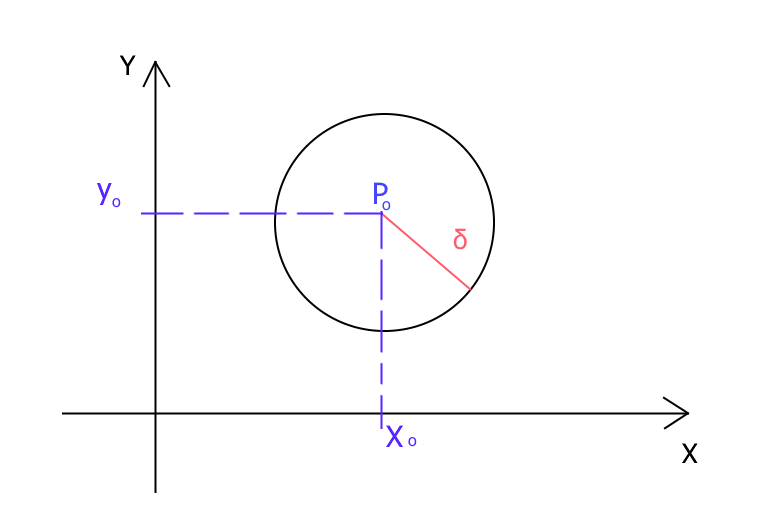
\includegraphics[width=\linewidth]{10img.png}

Окрестностью точки \(P_{0}\left(x_{0}; y_{0}\right)\) называется
внутренность круга с центром в этой точке. Радиус круга равен
\(\delta\). Очевидно, что любая точка \(P\left(x; y\right)\) \(\delta\)
- окрестности точки \(P_{0}\left(x_{0}; y_{0}\right)\) находится от этой
точки на расстоянии, меньшем \(\delta\).

\subsubsection{Определение.}

Число \(b\) называют пределом функции \(z=f(x, y)=f(P)\) при
\(P \rightarrow P_{0}\), если для
\(\forall \varepsilon>0 \quad \exists \delta\) - окрестность точки
\(P_{0}\left(x_{0}; y_{0}\right)\) , что для \(\forall\)
\(P\left(x; y\right)\) точки этой окресности, имеет место равенство:

\[
|f(P)-b|
<\varepsilon
\]

или \[
|f(x, y)-b|
<\varepsilon
\]

При этом пишут \(\lim _{P \rightarrow P_{0}} f(P)=b \quad\) или
\(\ \ \lim _{x \rightarrow x_{0} \atop y \rightarrow y_{0}} f(x, y)=b,\)
так как при \(P(x ; y) \rightarrow P_{0}\left(x_{0} ; y_{0}\right),\)
следует, \(x \rightarrow x_{0}, y \rightarrow y_{0}\) (в силу критерия
сходимости в пространстве \(\mathbb{R}^{n}\) )

\subsection{Повторный предел}

\subsubsection{Определение}

Для функции \(u=f\left(x_{1}, x_{2}, \ldots, x_{m}\right)\) нескольких
переменных можно определить понятие предела по одной из переменных
\(x_{k}\) при фиксированных значениях остальных переменных. В связи с
этим возникает понятие повторного предела. Уясним это понятие на примере
функции \(u=f(x, y)\). Пусть функция \(u=f(x, y)\) задана в некоторой
прямоугольной окрестности
\(0<\left|x-x_{0}\right|<d_{1},0<\left|y-y_{0}\right|<d_{2}\) точки
\(M_{0}\left(x_{0}, y_{0}\right)\), за исключением, быть может, самой
точки \(M_{0}\). Пусть для каждого фиксированного ``y'',
удовлетворяющего условию \(0<\left|y-y_{0}\right|<d_{2}\), существует
предел функции \(u=f(x, y)\) одной переменной \(x\) в точке \(x=x_{0}\):

\[\lim _{x \rightarrow x_{0} \atop y-\text {фикс }} f(x, y)=\varphi(y)\]

и пусть, кроме того, существует предел \(b\) функции \(\varphi(y)\) в
точке \(y=y_{0}\):

\[\lim _{y \rightarrow y_{0}} \varphi(y)=b\]

В этом случае говорят, что существует повторный предел \(b\) для функции
\(u=f(x, y)\) в точке \(M_{0}\), который обозначается следующим образом:

\[\lim _{y \rightarrow y_{0}} \lim _{x \rightarrow x_{0}} f(x, y)=b\]

Аналогично определяется повторный предел:

\[\lim _{x \rightarrow x_{0}} \lim _{y \rightarrow y_{0}} f(x, y)\]

\subsection{Теорема о связи двойных и повторных пределов}

Обратимся к вышеописанной функции \(u=f(x, y)\). Если:

\[\exists\lim _{x \rightarrow x_{0} \atop y \rightarrow y_{0} } f(x, y)=A\]

Пусть \(\forall\)\(x\): \(0<\left|x-x_{0}\right|<\delta_{1}\):
\[\exists\lim _{y \rightarrow y_{0}} f(x, y)=\varphi(x)\]

Тогда:

\[\exists\lim _{x \rightarrow x_{0}} \varphi(x)=A\]

Что равносильно:

\[\lim _{x \rightarrow x_{0}} \lim _{y \rightarrow y_{0}} f(x, y)=\lim _{x \rightarrow x_{0} \atop y \rightarrow y_{0}} f(x, y)=A\]

\subsubsection{Доказательство}

\(\forall \epsilon\)\textgreater{}0 \(\exists\)
\(\delta_{1}(\epsilon) > 0:\)
\(\forall M(x,y):\) \ \(0<\rho\)(\(M\),\(M_{0}\))\textless{}\(\delta_{1}\)
\(\Rightarrow\) \(\left|f(x,y)-A\right|<\epsilon/ 2\) \\

где: \(\rho\)(\(M\),\(M_{0}\)) = \(\max(|x-x_{0}|,| y-y_{0}|)\)
\(<\) \(\delta_{1}\) \\

\(\forall x:0<|x-x_{0}|<\delta:\)
\(\ \ \forall \epsilon\)\textgreater{}0\(:\)
\(\exists \delta_{2}(\epsilon,x)>0:\) \(\forall y:\)
\(0<\left|y-y_{0}\right|<\delta_{2}\) \(\Rightarrow\)
\(\left|f(x,y)-\varphi(x)\right|<\epsilon/ 2\) \\

\(\left|\varphi(x)-A\right|\leq\)
\(|f(x, y)-\varphi(x)|+| f(x, y)-A|\)\(<\) \(|f(x, y)-\varphi(x)|\) +
\(\epsilon/2<\) \(\epsilon/ 2\) + \(\epsilon/ 2\)=\(\epsilon\) \\

Ход преобразований: \\
1) Отнимем и прибавим функцию \(f(x,y)\) \\
2)\(| f(x, y)-A|\) \(< \epsilon /2\), если: \(\max(|x-x_{0}|,| y-y_{0}|)\)
\(<\) \(\delta_{1}\), следовательно сделаем условие для преобразования: \\

\[\left\{\begin{array}{l}
0<\left|x-x_{0}\right|<\delta_{1} \\
0<\left|y-y_{0}\right|<\delta_{1}
\end{array}\right.\]

\begin{enumerate}
\def\labelenumi{\arabic{enumi})}
\setcounter{enumi}{2}
\tightlist
\item
  \(|f(x, y)-\varphi(x)|\) \textless{} \(\epsilon /2\), если: \(x:\)
  \(0<\left|x-x_{0}\right|<\delta_{1}:\)
  \(\exists \delta_{2}(\epsilon, x)\), также условие для \textbf{y}:
\end{enumerate}

\[\left\{\begin{array}{l}
0<\left|y-y_{0}\right|<\delta_{2}(\epsilon, x) \\
0<\left|y-y_{0}\right|<\delta_{1}(\epsilon)
\end{array}\right.\]

\section{Определения непрерывности функции многих переменных по Коши и по Гейне.
Непрерывность на множестве.
Непрерывность в изолированной точке.}
\subsection{Определения непрерывности по Коши и по Гейне}
Пусть задана некоторая область $D \subseteq \mathbb{R}^m$ и для $ \forall x \in D \rightarrow \ ! y \in \mathbb{R}^{k}$, тогда функция определена на $D$, и $y=f(x)=f(x_{1}, x_{2}, ... , x_{n})$. Говорят, что функция $f$ - непрерывна в $a \in D$, если
$$
\exists \lim_{\substack{x_{1}\to a_{1}\\ ... \\{x_{n}\to a_{n}}}}{f(x_{1},..., x_{n})} = f(a_{1},..., a_{n})
$$
\textbf{по Гейне:}
$$
\forall x^{(n)} \in D, \ x^{(n)} \overset{\mathbb{R}^{m}}{\underset{n \rightarrow \infty}{\longrightarrow}} a \ \Rightarrow \
y^{(n)} = f(x^{(n)}) \rightarrow f(a) \in \mathbb{R}^{k}
$$
это означает, что какую бы последовательность векторов, сходящуюся к $a$, ни взять, соответствующая последовательность значений функции
$
f(x^{(1)}), f(x^{(2)}), ..., f(x^{(n)})
$
сходится к $f(a)$. \\
Стоит также уточнить, что если f - скалярная функция, то $f(a) \in \mathbb{R}$, а если f - вектор-функция, то есть
$$
f: D \in \mathbb{R}^{n} \rightarrow \mathbb{R}^{k}
$$
$$
x = (x_{1}, x_{2}, ... , x_{n}) \rightarrow y = (y_{1}, y_{2}, ... , y_{k})
$$
где
\begin{equation*}
y =
\begin{cases}
y_{1} =y_{1}(x_{1}, x_{2}, ... , x_{n}) \in \mathbb{R}\\
... \\
y_{k} =y_{k}(x_{1}, x_{2}, ... , x_{n}) \in \mathbb{R}
\end{cases}
\end{equation*}
- система k скалярных функций, то $f(a) \in \mathbb{R}^{k}$
\\\\
\textbf{по Коши:}
$$
\forall \varepsilon>0 \quad \exists \delta(\varepsilon)>0 :\ \forall x \in D \cap B(a, \delta)
\Rightarrow
$$
для скалярной функции: $|f(x) - f(a)| < \varepsilon$,
для вектор-функции: $f(x) \in B(a, \varepsilon)$.\\
Также можно записать и на языке метрик:
$$
\forall \varepsilon>0 \quad \exists \delta(\varepsilon)>0 \ \forall x \in D :\ \rho^{m}(x,a) < \delta
\Rightarrow \rho^{k}(f(x), f(a)) < \varepsilon
$$
\subsection{Непрерывность на множестве}
$f$ - непрерывна на некотором множестве $X$, если $f$ - непрерывна в каждой точке множества $X$

\subsection{Непрерывность в изолированной точке}
Всякая функция непрерывна в каждой изолированной точке множества своего определения.
\section{Основные свойства непрерывных функций. Устойчивость знака непрерывных функций}
\subsection{Основные свойства непрерывных функций.}
1. $f + g$ - непрерывна (в $\mathbb{R}^{k}$)\\
2. $f - g$ - непрерывна (в $\mathbb{R}^{k}$)\\
3. $f \cdot g$ - непрерывна (только в $\mathbb{R}$)\\
4. $f \over g$ - непрерывна (только в $\mathbb{R}$, если $g \neq 0 $) \\
5. сохранение знака непрерывной функции (только в $\mathbb{R}$)

\subsection{Устойчивость знака непрерывных функций.}
\textbf{Формулировка:}
Если $f(a) > 0 \ (f(a) < 0 )$ и $f$ - непрерывна в точке $a$, то найдутся такие $O(a)$ и $r>0$, что\\
$$
f(x) \geq r > 0 \ (f(x) \leq -r < 0)
$$
при $x \in O(a) \cap X$\\
\textbf{Доказательство:}\\
Если $a \in X$, то $\lim_{x\to a}{f(x)} = f(a)$, т.е
$$
\forall \varepsilon>0 \quad \exists \delta(\varepsilon)>0 \ \forall x \in O_{\delta}(a) \cap X
\Rightarrow |f(x)- f(a)| < \varepsilon
$$
Пусть $f(a)>0$. Положим $\varepsilon$ = ${f(a)\over 2} > 0$, по нему найдем $\delta(\varepsilon)$ и для любого $x \in O_{\delta}(a) \cap X$ получим
\begin{equation*}
\begin{gathered}
|f(x) - f(a)| < {f(a)\over 2}\\
f(a) - {f(a)\over 2} < f(x) < {3\over 2} f(a)\\
\end{gathered}
\end{equation*}
откуда
$$
f(x)> r = {f(a)\over 2} > 0
$$
\section{Понятие сложной функции. Теорема о непрерывности сложной функции.}

Теорема о непрерывности сложной функции. 
Пусть отображение $x = \phi (x)$ определено в некоторой окрестности точки $t_0 = (t^0_1, t^0_2, ..., t^0_m) \in R$ и непрерывным образом отображает ее в точку $x_0 = (x_1^0, x_2^0, ..., x_n^0) \in R^m$. Пусть функция \emph{f(x)} определена в некоторой окрестности точки $x_0$ и непрерывна в этой точке. Тогда сложная функция $F(t) = f(\phi (t))$ непрерывна в точке $t_0$.

\subsection{Доказательство}

Заметим, что для отображения 

\begin{displaymath}
    \phi (t) = (\phi _1(t), \phi _2(t), ..., \phi _n(t))
\end{displaymath}

непрерывность в точке $t_0$ означает непрерывность каждой из функций $\phi _i(t)$ в точке $t_0$ как функции m переменных, т.е. если $\{t^p\} \subset R^m$ и $t^p \underset{p \rightarrow \infty}{\longrightarrow} t_0$, то

\begin{displaymath}
    \phi (t^p) = (\phi _1(t^p), \phi _2(t^p), ..., \phi _n(t^p)) \underset{p \rightarrow \infty}{\longrightarrow} 
\end{displaymath}

\begin{displaymath}
    \underset{p \rightarrow \infty}{\longrightarrow} (\phi _1(t_0), \phi _2(t_0), ..., \phi _n(t_0)) = (x_1^0, x_2^0, ..., x_n^0) = x_0.
\end{displaymath}

Положим $x^p = \phi (t^p)$, тогда $x^p \underset{p \rightarrow \infty}{\longrightarrow} x_0$. В силу непрерывности функции $f$, $f(x^p) \underset{p \rightarrow \infty}{\longrightarrow} f(x_0)$, т.е. 

\begin{displaymath}
    F(t^p) = f(\phi (t^p)) \underset{p \rightarrow \infty}{ \longrightarrow} f(x_0) = f(\phi (t_0)) = F(t_0)
\end{displaymath}
\end{document}
